\section{对称性}

\subsection{守恒量}

迄今为止我们已经研究过空间平移对称、时间平移对称和旋转对称。这些对称操作可用一个(或一组)连续参量来表示,参量取值与对称操作有一一对应的关系,参量的连续变化描述了群元的连续变化,如此构成的群是个连续群。群元乘积的参量是每个操作参量的单值解析函数,这样的连续群称为李群(Lie Group)。这里我们只是提及这些名词,并不深入数学上的细节。

我们用一个幺正算符$U$来表示对称操作中的一个元素,对无穷小参量$\epsilon$,可统一写成如下形式:

\begin{equation}
U(\epsilon) = 1 - \frac{i \epsilon G}{\hbar}
\end{equation}

$G^\dagger = G$是厄米算符,是对称算符的产生算符,因为我们只要让很多无穷小算符连乘就可得到有限参量的对称操作。$G$可以是$p_x$,$H$或$J_z$,对应的无穷小参量是$\delta x$,$\delta t$和$\delta \phi$。

在对称操作$U$下,态矢量$\left| \alpha \right\rangle \to U \left| \alpha \right\rangle $,假设在对称操作$U$下,哈密顿$H$是不变的。这意味着:

\begin{equation}
\left\langle \alpha \right| H \left| \alpha \right\rangle = \left\langle \alpha \right| U^\dagger H U \left| \alpha \right\rangle 
\end{equation}

即:$H = U^\dagger H U$,那么:$U H = H U $,那么:

\begin{equation*}
\left( 1 - \frac{i \epsilon G}{\hbar} \right) H = H \left( 1 - \frac{i \epsilon G}{\hbar} \right)
\end{equation*}

这意味着:

\begin{equation}
[G, H ] = 0
\end{equation}

考虑海森堡运动方程\index{Heisenberg equation of motion:海森堡运动方程}:

\begin{equation}
i \hbar \dot G = [G, H ] = 0
\end{equation}

这意味着力学量$G$是守恒量。即空间平移对称对应“动量守恒”,时间平移对称对应“能量守恒”,而转动对称对应“角动量守恒”。

假设$\left| n \right\rangle$是$H$的本征态,对应的本征值是$E_n$

\begin{equation}
H \left| n \right\rangle = E_n \left| n \right\rangle
\end{equation}

由于$ HU = UH$,

\begin{equation}
H U \left| n \right\rangle = U H \left| n \right\rangle = E_n U \left| n \right\rangle 
\end{equation}

即$U \left| n \right\rangle $和$\left| n \right\rangle$都对应相同的能量本征值$E_n$,如果$U \left| n \right\rangle $和$\left| n \right\rangle$是两个不同的量子态,我们就说$E_n$是简并的。

\subsection{宇称}

除了连续的对称操作,还有分立的对称操作。比如宇称\index{Parity:宇称}(parity,也叫空间反演),

\begin{equation}
\left| \alpha \right\rangle \to \pi \left| \alpha \right\rangle
\end{equation}

使得:

\begin{equation}
\left\langle x \right\rangle \to  \left\langle \alpha \right| \pi^\dagger x \pi \left| \alpha \right\rangle   =  - \left\langle  \alpha \right|  x \left| \alpha \right\rangle 
\end{equation}

这意味着:

\begin{equation}
\pi^\dagger x \pi = - x 
\end{equation}

我们说位置矢量$x$在宇称变换下是奇(odd)的。

现在考虑如图操作:

\begin{figure}[htbp]
\begin{center}
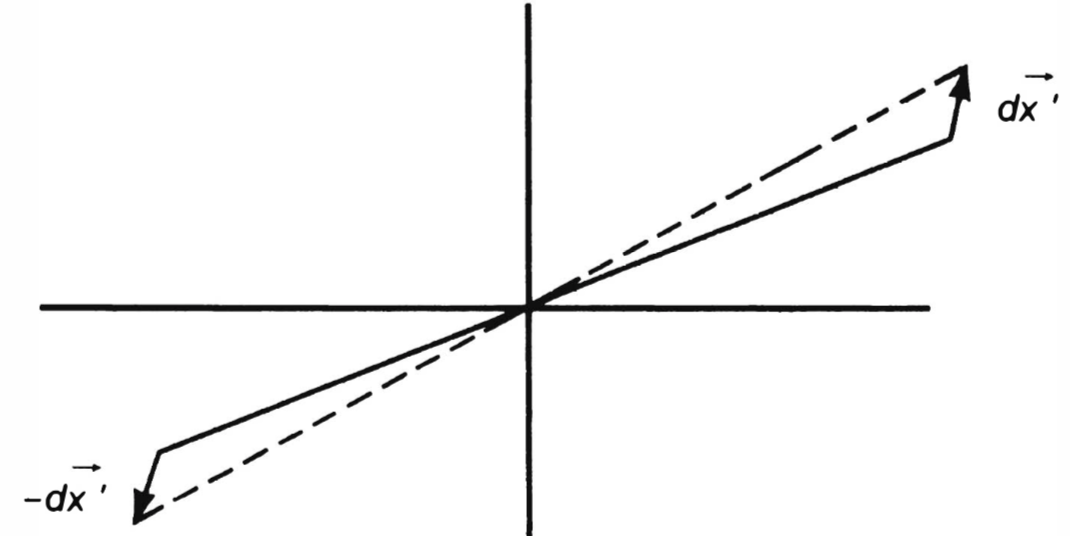
\includegraphics[width=9cm]{Symmetry/piTTpi.png}
\caption{$\pi T(dx') = T(- dx') \pi$}
%\label{default}
\end{center}
\end{figure}

先平移$T(dx')$再宇称(空间反演\index{inversion:空间反演},inversion)$\pi$的效果$\pi T(dx')$和先宇称$\pi$再反方向平移$T(- dx')$的效果$ T(- dx') \pi$是一样的。记作:

\begin{equation}
\pi T(dx') = T(- dx') \pi
\end{equation}

这意味着:

\begin{equation}
\pi \left( 1 - \frac{i p dx'}{\hbar}   \right) = \left( 1 + \frac{i p dx'}{\hbar}   \right) \pi
\end{equation}

即:

\begin{equation}
\pi^\dagger p \pi = - p
\end{equation}

动量算符在宇称变换下也是奇(odd)的。

现在来考虑角动量算符$J$,对轨道角动量$L = x \times p$,我们猜测角动量在宇称变换下是偶(even)的。

在三维实空间,空间反演(即宇称变换)可写为:

\begin{equation}
R(\pi) = \left( \begin{array}{ccc} -1 & 0 & 0 \\ 0 & -1 & 0 \\ 0 & 0 & -1  \end{array}  \right)
\end{equation}

$R(\pi)$与实空间中的任意转动$R_{n} (\phi)$对易:

\begin{equation}
R(\pi) R_{n} (\phi) = R_{n} (\phi) R(\pi)
\end{equation}

对应到态矢空间中的变换矩阵应有相同的关系:

\begin{equation}
\pi D(R) = D(R) \pi
\end{equation}

这意味着:

\begin{equation}
\pi \left( 1- \frac{i J_n d \phi}{\hbar}  \right) = \left( 1- \frac{i J_n d \phi}{\hbar}  \right) \pi
\end{equation}

即:

\begin{equation}
\pi^\dagger J_n \pi = J_n 
\end{equation}

我们称$x$,$p$这样的向量叫极向量\index{polar vector:极向量}(polar vector),而称像角动量$J$这样的向量为轴向量\index{axial vector:轴向量}(axial vector),或赝向量\index{pseudovector:赝向量}(pseudovector)。在此基础上我们可继续定义标量,如$L \cdot S$和赝标量\index{pseudoscalar:赝标量}$S \cdot x$。

\begin{eqnarray}
\pi^\dagger L \cdot S  \pi & = & L \cdot S \\
\pi^\dagger  S \cdot x  \pi & = & - S \cdot x
\end{eqnarray}

练习:假设$[H, \pi] = 0$(哈密顿具有宇称对称),假设$\left| n \right\rangle$是$H$的非简并本征态(nondegenerate eigenket),对应本征值是$E_n$,求证$\left| n \right\rangle$也是宇称算符$\pi$的本征态。

Prove:首先构造态矢量

\begin{equation}
\frac{ \left| n \right\rangle \pm \pi \left| n \right\rangle }{2}
\end{equation}

它是宇称算符的本征态,

\begin{equation}
\pi \left( \frac{ \left| n \right\rangle \pm \pi \left| n \right\rangle }{2}  \right) = \frac{ \pi \left| n \right\rangle \pm \left| n \right\rangle }{2} = \pm \frac{\left| n \right\rangle \pm \pi \left| n \right\rangle}{2}
\end{equation}

其本征值是$\pm 1$,并且这个态对应能量本征值仍然是$E_n$:

\begin{equation}
H \frac{ \left| n \right\rangle \pm \pi \left| n \right\rangle }{2} = E_n \frac{ \left| n \right\rangle \pm \pi \left| n \right\rangle }{2}
\end{equation}

由于$E_n$非简并,$\frac{ \left| n \right\rangle \pm \pi \left| n \right\rangle }{2}$实际上和$\left| n \right\rangle$是一个态(可以相差一个相位因子)。

\subsection{对称双井}

考虑如图“左右对称”的双井,它符合上述$[ H, \pi ] = 0$的条件,其能量本征态$\left| n \right\rangle$具有确定的奇偶性。考虑能量最低“偶宇称”的态$\left| S \right\rangle$,其能量本征值是$E_S$,和能量最低“奇宇称”的态$\left| A \right\rangle$,其能量本征值是$E_A$。

\begin{figure}[htbp]
\begin{center}
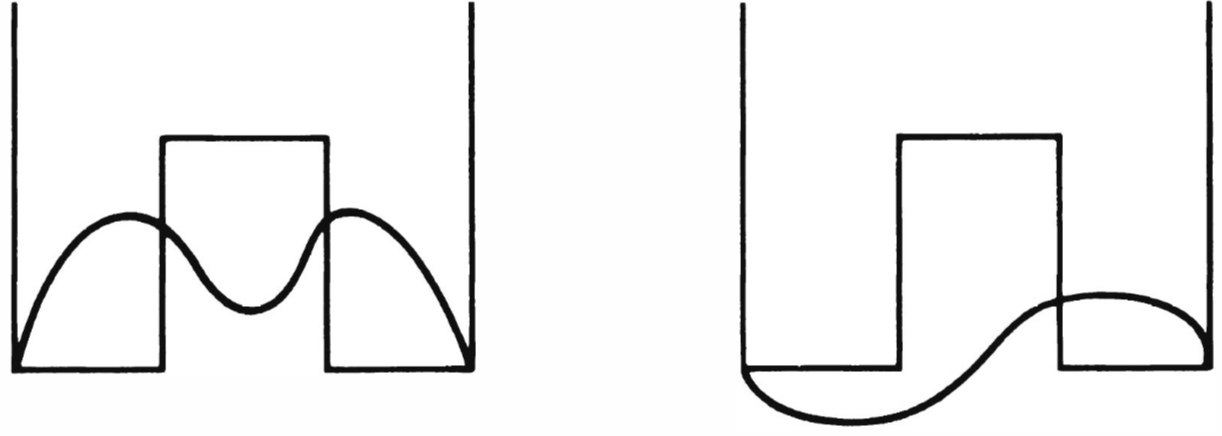
\includegraphics[width=8cm]{Symmetry/symmetry-antisymmetry.png}
\caption{左:偶宇称的态;右:奇宇称的态。}
%\label{default}
\end{center}
\end{figure}

由于奇宇称的态$\left| A \right\rangle$起伏更激烈,所以有

\begin{equation}
E_A > E_S
\end{equation}

假设对称双井中间的势垒较高,即$\left| S \right\rangle$和$\left| A \right\rangle$在左井和右井中“波函数的形状”大致相同。这样我们可以把$\left| S \right\rangle$和$\left| A \right\rangle$组合起来分别得到局域在右井和左井中的态矢量$\left| R \right\rangle$和$\left| L \right\rangle$:

\begin{eqnarray}
\left| R \right\rangle  & = & \frac{ \left| S \right\rangle + \left| A \right\rangle  }{\sqrt{2}} \\
\left| L \right\rangle & = & \frac{ \left| S \right\rangle - \left| A \right\rangle  }{\sqrt{2}}
\end{eqnarray}

假设$t=0$,粒子处于右井中,即$\left| R, t=0 \right\rangle$,态矢量将如何演化?考虑:

\begin{eqnarray*}
\left| R , t \right\rangle & = & e^{- \frac{iHt}{\hbar}}  \left| R \right\rangle =  \frac{ e^{- \frac{iHt}{\hbar}} \left| S \right\rangle + e^{- \frac{iHt}{\hbar}} \left| A \right\rangle   }{\sqrt 2} \\
{} & = & \frac{ e^{- \frac{iE_S t}{\hbar}} \left| S \right\rangle + e^{- \frac{i E_A t}{\hbar}} \left| A \right\rangle   }{\sqrt 2} \\
{} & = & \frac{1}{\sqrt 2} e^{ - \frac{i E_S t}{ \hbar} } \left( \left| S \right\rangle + e^{- \frac{i (E_A - E_S) t }{ \hbar}}  \left| A \right\rangle  \right)
\end{eqnarray*}

由上式括号中第二项可看出,每经历半周期$\left| R \right\rangle \to \left| L \right\rangle $,再经历半周期$\left| L \right\rangle \to \left| R \right\rangle $,即粒子会经历从右井到左井,再从左井回到右井的反复周期振荡。振荡周期为:

\begin{equation}
T = \frac{h }{E_A - E_S}
\end{equation}

由上式可见,$E_A$和$E_S$越接近,粒子由右井振荡到左井的时间就越久,如果$E_A$无限趋近于$E_S$,粒子就会“永远”呆在右井。对应就是对称双井中间的势垒趋于无限高的情形。

\begin{figure}[htbp]
\begin{center}
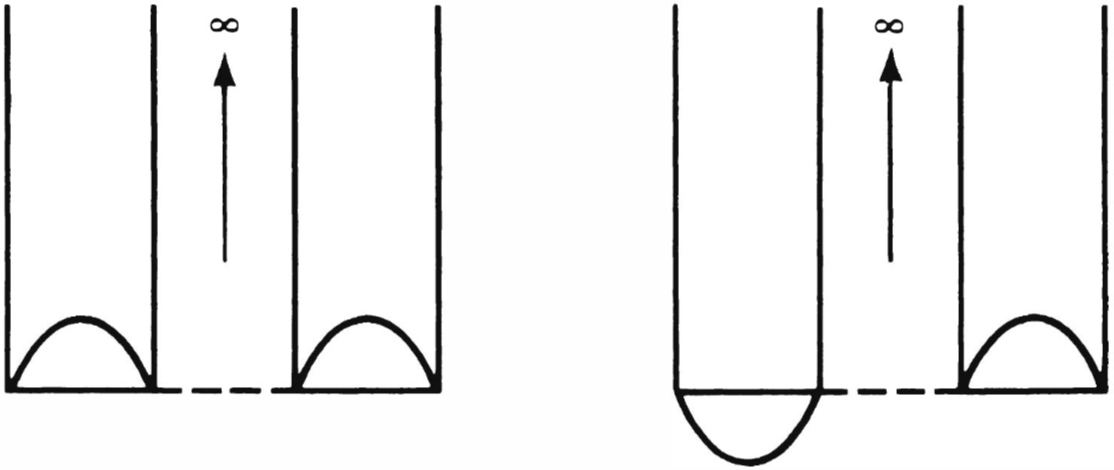
\includegraphics[width=8cm]{Symmetry/infinitedoublewell.png}
\caption{中间势垒趋于无穷高的对称双井}
%\label{default}
\end{center}
\end{figure}

对称双井可用于描述氨分子振荡。氨分子中的N原子可以在三个H原子的上面,也可在三个H原子的下面。N原子和三个H原子组成金字塔,N原子是塔尖,三个H原子构成金字塔的底面。氨分子整体可围绕通过塔尖和底面中心的轴转动,塔尖(N)是否在底面($H_3$)的上面是相对于这个转动而言的。由于氨分子中正、负电荷中心不重合,N端稍带负电,$H_3$端稍带正电,氨分子整体有非零的电偶极矩\index{electric dipole moment:电偶极矩}(electric dipole moment),由N指向$H_3$。

\begin{figure}[htbp]
\begin{center}
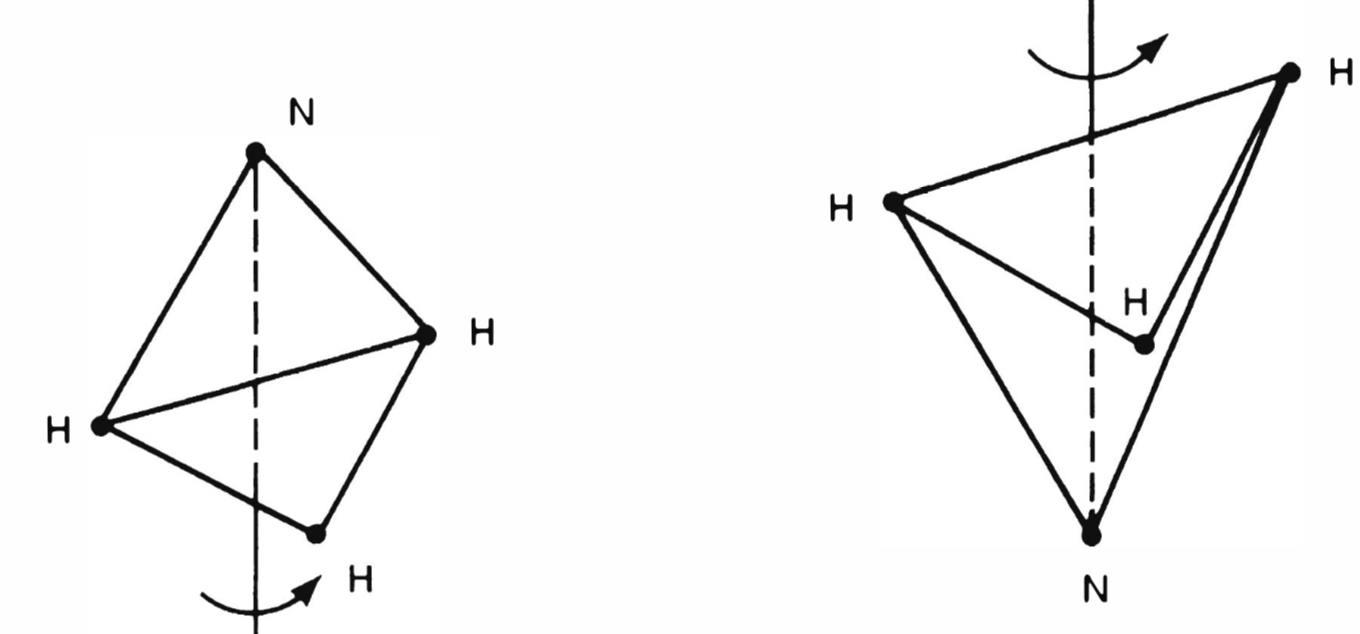
\includegraphics[width=9cm]{Symmetry/amoniamolecule.png}
\caption{氨分子}
%\label{default}
\end{center}
\end{figure}

氨分子对称构型和反对称构型的能量差($\approx  \times 10^{-4} eV$)对应的频率是$24000$MHz,对应波长是1cm。对应电磁波谱中的微波。对$PH_3$而言,它具有和$NH_3$类似的结构,但P比N更难“隧穿”$H_3$平面,频率只有$NH_3$的十分之一。对更重的$PF_3$,我们甚至无法测量到P“隧穿”$F_3$平面的频率。

\subsection*{参考}

J. J. Sakurai, Modern Quantum Mechanics, \S 4.1, 4.2

P. W. Anderson, More is Different, Science, New Series, Vol. 177, No. 4047 (Aug 4, 1972), pp393-396